\documentclass[twoside]{book}

% Packages required by doxygen
\usepackage{fixltx2e}
\usepackage{calc}
\usepackage{doxygen}
\usepackage[export]{adjustbox} % also loads graphicx
\usepackage{graphicx}
\usepackage[utf8]{inputenc}
\usepackage{makeidx}
\usepackage{multicol}
\usepackage{multirow}
\PassOptionsToPackage{warn}{textcomp}
\usepackage{textcomp}
\usepackage[nointegrals]{wasysym}
\usepackage[table]{xcolor}

% Font selection
\usepackage[T1]{fontenc}
\usepackage[scaled=.90]{helvet}
\usepackage{courier}
\usepackage{amssymb}
\usepackage{sectsty}
\renewcommand{\familydefault}{\sfdefault}
\allsectionsfont{%
  \fontseries{bc}\selectfont%
  \color{darkgray}%
}
\renewcommand{\DoxyLabelFont}{%
  \fontseries{bc}\selectfont%
  \color{darkgray}%
}
\newcommand{\+}{\discretionary{\mbox{\scriptsize$\hookleftarrow$}}{}{}}

% Page & text layout
\usepackage{geometry}
\geometry{%
  a4paper,%
  top=2.5cm,%
  bottom=2.5cm,%
  left=2.5cm,%
  right=2.5cm%
}
\tolerance=750
\hfuzz=15pt
\hbadness=750
\setlength{\emergencystretch}{15pt}
\setlength{\parindent}{0cm}
\setlength{\parskip}{3ex plus 2ex minus 2ex}
\makeatletter
\renewcommand{\paragraph}{%
  \@startsection{paragraph}{4}{0ex}{-1.0ex}{1.0ex}{%
    \normalfont\normalsize\bfseries\SS@parafont%
  }%
}
\renewcommand{\subparagraph}{%
  \@startsection{subparagraph}{5}{0ex}{-1.0ex}{1.0ex}{%
    \normalfont\normalsize\bfseries\SS@subparafont%
  }%
}
\makeatother

% Headers & footers
\usepackage{fancyhdr}
\pagestyle{fancyplain}
\fancyhead[LE]{\fancyplain{}{\bfseries\thepage}}
\fancyhead[CE]{\fancyplain{}{}}
\fancyhead[RE]{\fancyplain{}{\bfseries\leftmark}}
\fancyhead[LO]{\fancyplain{}{\bfseries\rightmark}}
\fancyhead[CO]{\fancyplain{}{}}
\fancyhead[RO]{\fancyplain{}{\bfseries\thepage}}
\fancyfoot[LE]{\fancyplain{}{}}
\fancyfoot[CE]{\fancyplain{}{}}
\fancyfoot[RE]{\fancyplain{}{\bfseries\scriptsize Generated by Doxygen }}
\fancyfoot[LO]{\fancyplain{}{\bfseries\scriptsize Generated by Doxygen }}
\fancyfoot[CO]{\fancyplain{}{}}
\fancyfoot[RO]{\fancyplain{}{}}
\renewcommand{\footrulewidth}{0.4pt}
\renewcommand{\chaptermark}[1]{%
  \markboth{#1}{}%
}
\renewcommand{\sectionmark}[1]{%
  \markright{\thesection\ #1}%
}

% Indices & bibliography
\usepackage{natbib}
\usepackage[titles]{tocloft}
\setcounter{tocdepth}{3}
\setcounter{secnumdepth}{5}
\makeindex

% Hyperlinks (required, but should be loaded last)
\usepackage{ifpdf}
\ifpdf
  \usepackage[pdftex,pagebackref=true]{hyperref}
\else
  \usepackage[ps2pdf,pagebackref=true]{hyperref}
\fi
\hypersetup{%
  colorlinks=true,%
  linkcolor=blue,%
  citecolor=blue,%
  unicode%
}

% Custom commands
\newcommand{\clearemptydoublepage}{%
  \newpage{\pagestyle{empty}\cleardoublepage}%
}

\usepackage{caption}
\captionsetup{labelsep=space,justification=centering,font={bf},singlelinecheck=off,skip=4pt,position=top}

%===== C O N T E N T S =====

\begin{document}

% Titlepage & ToC
\hypersetup{pageanchor=false,
             bookmarksnumbered=true,
             pdfencoding=unicode
            }
\pagenumbering{alph}
\begin{titlepage}
\vspace*{7cm}
\begin{center}%
{\Large M\+\_\+readline }\\
\vspace*{1cm}
{\large Generated by Doxygen 1.8.14}\\
\end{center}
\end{titlepage}
\clearemptydoublepage
\pagenumbering{roman}
\tableofcontents
\clearemptydoublepage
\pagenumbering{arabic}
\hypersetup{pageanchor=true}

%--- Begin generated contents ---
\chapter{M\+\_\+readline Fortran Library}
\label{index}\hypertarget{index}{}\hypertarget{index_Introduction}{}\section{Introduction}\label{index_Introduction}
M\+\_\+readline -\/ Fortran module to interface with readline(3c) \begin{DoxyVerb}@image html html/images/yarnball.gif\end{DoxyVerb}
 
\chapter{Modules Index}
\doxysection{Modules List}
Here is a list of all modules with brief descriptions\+:\begin{DoxyCompactList}
\item\contentsline{section}{\mbox{\hyperlink{namespacem__readline}{m\+\_\+readline}} }{\pageref{namespacem__readline}}{}
\end{DoxyCompactList}

\chapter{Data Type Index}
\doxysection{Data Types List}
Here are the data types with brief descriptions\+:\begin{DoxyCompactList}
\item\contentsline{section}{\mbox{\hyperlink{interfacem__readline_1_1Freadline}{m\+\_\+readline\+::\+Freadline}} }{\pageref{interfacem__readline_1_1Freadline}}{}
\end{DoxyCompactList}

\chapter{File Index}
\doxysection{File List}
Here is a list of all files with brief descriptions\+:\begin{DoxyCompactList}
\item\contentsline{section}{/home/urbanjs/venus/\+V600/github/\+C\+W\+R\+A\+P/\+M\+\_\+readline/src/\mbox{\hyperlink{C-M__readline_8c}{C-\/\+M\+\_\+readline.\+c}} }{\pageref{C-M__readline_8c}}{}
\item\contentsline{section}{/home/urbanjs/venus/\+V600/github/\+C\+W\+R\+A\+P/\+M\+\_\+readline/src/\mbox{\hyperlink{M__readline_8f90}{M\+\_\+readline.\+f90}} }{\pageref{M__readline_8f90}}{}
\end{DoxyCompactList}

\chapter{Module Documentation}
\hypertarget{namespacem__readline}{}\doxysection{m\+\_\+readline Module Reference}
\label{namespacem__readline}\index{m\_readline@{m\_readline}}
\doxysubsection*{Data Types}
\begin{DoxyCompactItemize}
\item 
interface \mbox{\hyperlink{interfacem__readline_1_1Freadline}{Freadline}}
\end{DoxyCompactItemize}
\doxysubsection*{Functions/\+Subroutines}
\begin{DoxyCompactItemize}
\item 
subroutine, public \mbox{\hyperlink{namespacem__readline_a6eae368d34bd43ead64623b2d6d10ae0}{system\+\_\+readline}} (line, prompt)
\end{DoxyCompactItemize}


\doxysubsection{Detailed Description}
\hypertarget{namespacem__readline_autotoc_md0}{}\doxysubsubsection{N\+A\+ME}\label{namespacem__readline_autotoc_md0}
M\+\_\+readline(3fm) -\/ \mbox{[}M\+\_\+readline\+::\+I\+N\+T\+RO\mbox{]} Calling readline(3c) from Fortran (L\+I\+C\+E\+N\+SE\+:PD) \hypertarget{namespacem__readline_autotoc_md1}{}\doxysubsubsection{S\+Y\+N\+O\+P\+S\+IS}\label{namespacem__readline_autotoc_md1}
\begin{DoxyVerb}  Use M_readline, only : system_readline
\end{DoxyVerb}
 \hypertarget{namespacem__readline_autotoc_md2}{}\doxysubsubsection{D\+E\+S\+C\+R\+I\+P\+T\+I\+ON}\label{namespacem__readline_autotoc_md2}
\begin{DoxyVerb}The M_readline(3fm) module uses the ISO_C_BINDING module to create a
binding to the GNU readline(3c) procedure from Fortran programs.
\end{DoxyVerb}
\hypertarget{namespacem__readline_autotoc_md3}{}\doxysubsubsection{E\+X\+A\+M\+P\+LE}\label{namespacem__readline_autotoc_md3}
\begin{DoxyVerb}The test program is basically just a read loop that prompts for
lines of input read with readline(3c). You can edit the line being
read with readline(3c) per its documentation. At a minimum, you can
probably move around the line with the left and right arrow keys, and
insert characters by typing them wherever you moved the cursor to,
and use the DEL/ RUBOUT key to delete characters and such. If you use
a GNU/Linux shell with command line editing, you are probably familiar
with readline(3c)'s function.

It quits if you enter 'q' on an input line, and it dumps the history if
you enter 'h'.
\end{DoxyVerb}


the test program

program demo\+\_\+\+M\+\_\+readline use M\+\_\+readline implicit none character(len=256)\+:: line integer \+:: cstat character(len=256) \+:: sstat

write($\ast$,$\ast$)\textquotesingle{} \+\_\+\+\_\+\+\_\+\+\_\+\+\_\+\+\_\+\+\_\+\+\_\+\+\_\+\+\_\+\+\_\+\+\_\+\+\_\+\+\_\+\+\_\+\+\_\+\+\_\+\+\_\+\+\_\+\+\_\+\+\_\+\+\_\+\+\_\+\+\_\+\+\_\+\+\_\+\+\_\+\+\_\+\+\_\+\+\_\+\+\_\+\+\_\+\+\_\+\+\_\+\+\_\+\+\_\+\+\_\+\+\_\+\+\_\+\+\_\+\+\_\+\+\_\+\+\_\+\+\_\+\+\_\+\+\_\+\+\_\+\+\_\+\+\_\+\+\_\+\+\_\+\+\_\+\+\_\+\+\_\+\+\_\+\+\_\+\+\_\+\+\_\+\+\_\+\+\_\+\textquotesingle{} write($\ast$,$\ast$)\textquotesingle{} Your input lines are now editable using the G\+NU\textquotesingle{} write($\ast$,$\ast$)\textquotesingle{} readline(3\+C) procedure. By default, up-\/arrow and\textquotesingle{} write($\ast$,$\ast$)\textquotesingle{} down-\/arrow go thru the history lines; left and right arrow\textquotesingle{} write($\ast$,$\ast$)\textquotesingle{} keys and delete and just typing characters let you do\textquotesingle{} write($\ast$,$\ast$)\textquotesingle{} simple editing. Far more input control is available.\textquotesingle{} write($\ast$,$\ast$)\textquotesingle{} See the browser pages and man(1) pages for readline(3c).\textquotesingle{} write($\ast$,$\ast$)\textquotesingle{} \+\_\+\+\_\+\+\_\+\+\_\+\+\_\+\+\_\+\+\_\+\+\_\+\+\_\+\+\_\+\+\_\+\+\_\+\+\_\+\+\_\+\+\_\+\+\_\+\+\_\+\+\_\+\+\_\+\+\_\+\+\_\+\+\_\+\+\_\+\+\_\+\+\_\+\+\_\+\+\_\+\+\_\+\+\_\+\+\_\+\+\_\+\+\_\+\+\_\+\+\_\+\+\_\+\+\_\+\+\_\+\+\_\+\+\_\+\+\_\+\+\_\+\+\_\+\+\_\+\+\_\+\+\_\+\+\_\+\+\_\+\+\_\+\+\_\+\+\_\+\+\_\+\+\_\+\+\_\+\+\_\+\+\_\+\+\_\+\+\_\+\+\_\+\+\_\+\+\_\+\textquotesingle{} write($\ast$,$\ast$)\textquotesingle{} Enter text and then edit it. \char`\"{}q\char`\"{} quits; \char`\"{}h\char`\"{} display history\+:\textquotesingle{}

do call system\+\_\+readline(line,\textquotesingle{}readline$>$\textquotesingle{}) ! read editable input line if(line.\+eq.\textquotesingle{}q\textquotesingle{}) stop !call system(trim(line)) ! common extension call execute\+\_\+command\+\_\+line(trim(line),cmdstat=cstat,cmdmsg=sstat) ! f08 equivalent enddo end program demo\+\_\+\+M\+\_\+readline \hypertarget{namespacem__readline_autotoc_md4}{}\doxysubsubsection{A\+U\+T\+H\+OR}\label{namespacem__readline_autotoc_md4}
John S. Urban \hypertarget{namespacem__readline_autotoc_md5}{}\doxysubsubsection{L\+I\+C\+E\+N\+SE}\label{namespacem__readline_autotoc_md5}
Public Domain

Although this interface to readline(3c) is released as Public Domain, note that the Readline library itself is free software, distributed under the terms of the \mbox{[}G\+NU\mbox{]} General Public License, version 2. 

\doxysubsection{Function/\+Subroutine Documentation}
\mbox{\Hypertarget{namespacem__readline_a6eae368d34bd43ead64623b2d6d10ae0}\label{namespacem__readline_a6eae368d34bd43ead64623b2d6d10ae0}} 
\index{m\_readline@{m\_readline}!system\_readline@{system\_readline}}
\index{system\_readline@{system\_readline}!m\_readline@{m\_readline}}
\doxysubsubsection{\texorpdfstring{system\_readline()}{system\_readline()}}
{\footnotesize\ttfamily subroutine, public m\+\_\+readline\+::system\+\_\+readline (\begin{DoxyParamCaption}\item[{character(kind=c\+\_\+char,len=$\ast$), intent(out)}]{line,  }\item[{character(kind=c\+\_\+char,len=$\ast$), intent(in)}]{prompt }\end{DoxyParamCaption})}

\hypertarget{namespacem__readline_autotoc_md6}{}\doxysubsubsection{N\+A\+ME}\label{namespacem__readline_autotoc_md6}
system\+\_\+readline(3f) -\/ \mbox{[}M\+\_\+readline\mbox{]} Call readline(3c) from Fortran (L\+I\+C\+E\+N\+SE\+:PD) \hypertarget{namespacem__readline_autotoc_md7}{}\doxysubsubsection{S\+Y\+N\+O\+P\+S\+IS}\label{namespacem__readline_autotoc_md7}
\begin{DoxyVerb} character(kind=c_char,len=*),intent(in) :: prompt
 character(kind=c_char,len=*),intent(out) :: line
\end{DoxyVerb}
\hypertarget{namespacem__readline_autotoc_md8}{}\doxysubsubsection{D\+E\+S\+C\+R\+I\+P\+T\+I\+ON}\label{namespacem__readline_autotoc_md8}
\begin{DoxyVerb}The system_readline(3f) uses the ISO_C_BINDING module to create a
binding to the GNU readline(3c) procedure from Fortran programs.
\end{DoxyVerb}
\hypertarget{namespacem__readline_autotoc_md9}{}\doxysubsubsection{E\+X\+A\+M\+P\+LE}\label{namespacem__readline_autotoc_md9}
\begin{DoxyVerb}The test program is basically just a read loop that prompts for
lines of input read with readline(3c). You can edit the line being
read with readline(3c) per its documentation. At a minimum, you can
probably move around the line with the left and right arrow keys, and
insert characters by typing them wherever you moved the cursor to,
and use the DEL/ RUBOUT key to delete characters and such. If you use
a GNU/Linux shell with command line editing, you are probably familiar
with readline(3c)'s function.

It quits if you enter 'q' on an input line, and it dumps the history if
you enter 'h'.

It is presented here as a Bourne shell script that creates the necessary
files and does a "compile, load, and go"
\end{DoxyVerb}


the test program

program demo\+\_\+system\+\_\+readline use \mbox{\hyperlink{namespacem__readline}{m\+\_\+readline}}, only \+: system\+\_\+readline implicit none character(len=256) \+:: line integer \+:: cstat character(len=256) \+:: sstat

write($\ast$,$\ast$)\textquotesingle{} \+\_\+\+\_\+\+\_\+\+\_\+\+\_\+\+\_\+\+\_\+\+\_\+\+\_\+\+\_\+\+\_\+\+\_\+\+\_\+\+\_\+\+\_\+\+\_\+\+\_\+\+\_\+\+\_\+\+\_\+\+\_\+\+\_\+\+\_\+\+\_\+\+\_\+\+\_\+\+\_\+\+\_\+\+\_\+\+\_\+\+\_\+\+\_\+\+\_\+\+\_\+\+\_\+\+\_\+\+\_\+\+\_\+\+\_\+\+\_\+\+\_\+\+\_\+\+\_\+\+\_\+\+\_\+\+\_\+\+\_\+\+\_\+\+\_\+\+\_\+\+\_\+\+\_\+\+\_\+\+\_\+\+\_\+\+\_\+\+\_\+\+\_\+\+\_\+\+\_\+\textquotesingle{} write($\ast$,$\ast$)\textquotesingle{} Your input lines are now editable using the G\+NU\textquotesingle{} write($\ast$,$\ast$)\textquotesingle{} readline(3\+C) procedure. By default, up-\/arrow and\textquotesingle{} write($\ast$,$\ast$)\textquotesingle{} down-\/arrow go thru the history lines; left and right arrow\textquotesingle{} write($\ast$,$\ast$)\textquotesingle{} keys and delete and just typing characters let you do\textquotesingle{} write($\ast$,$\ast$)\textquotesingle{} simple editing. Far more input control is available.\textquotesingle{} write($\ast$,$\ast$)\textquotesingle{} See the browser pages and man(1) pages for readline(3c).\textquotesingle{} write($\ast$,$\ast$)\textquotesingle{} \+\_\+\+\_\+\+\_\+\+\_\+\+\_\+\+\_\+\+\_\+\+\_\+\+\_\+\+\_\+\+\_\+\+\_\+\+\_\+\+\_\+\+\_\+\+\_\+\+\_\+\+\_\+\+\_\+\+\_\+\+\_\+\+\_\+\+\_\+\+\_\+\+\_\+\+\_\+\+\_\+\+\_\+\+\_\+\+\_\+\+\_\+\+\_\+\+\_\+\+\_\+\+\_\+\+\_\+\+\_\+\+\_\+\+\_\+\+\_\+\+\_\+\+\_\+\+\_\+\+\_\+\+\_\+\+\_\+\+\_\+\+\_\+\+\_\+\+\_\+\+\_\+\+\_\+\+\_\+\+\_\+\+\_\+\+\_\+\+\_\+\+\_\+\+\_\+\+\_\+\textquotesingle{} write($\ast$,$\ast$)\textquotesingle{} Enter text and then edit it. \char`\"{}q\char`\"{} quits; \char`\"{}h\char`\"{} display history\+:\textquotesingle{}

do call system\+\_\+readline(line,\textquotesingle{}readline$>$\textquotesingle{}) ! read editable input line if(line.\+eq.\textquotesingle{}q\textquotesingle{}) stop call execute\+\_\+command\+\_\+line(trim(line),cmdstat=cstat,cmdmsg=sstat) enddo end program demo\+\_\+system\+\_\+readline \hypertarget{namespacem__readline_autotoc_md10}{}\doxysubsubsection{A\+U\+T\+H\+OR}\label{namespacem__readline_autotoc_md10}
John S. Urban \hypertarget{namespacem__readline_autotoc_md11}{}\doxysubsubsection{L\+I\+C\+E\+N\+SE}\label{namespacem__readline_autotoc_md11}
Public Domain

Although this interface to readline(3c) is released as Public Domain, note that the Readline library itself is free software, distributed under the terms of the \mbox{[}G\+NU\mbox{]} General Public License, version 2. 
\chapter{Data Type Documentation}
\hypertarget{interfacem__readline_1_1Freadline}{}\section{m\+\_\+readline\+:\+:Freadline Interface Reference}
\label{interfacem__readline_1_1Freadline}\index{m\+\_\+readline\+::\+Freadline@{m\+\_\+readline\+::\+Freadline}}
\subsection*{Private Member Functions}
\begin{DoxyCompactItemize}
\item 
subroutine \mbox{\hyperlink{interfacem__readline_1_1Freadline_ae441234495ff8c5daae930cd6ea51115}{freadline}} (ilen, buf, prompt)
\end{DoxyCompactItemize}


\subsection{Member Function/\+Subroutine Documentation}
\mbox{\Hypertarget{interfacem__readline_1_1Freadline_ae441234495ff8c5daae930cd6ea51115}\label{interfacem__readline_1_1Freadline_ae441234495ff8c5daae930cd6ea51115}} 
\index{m\+\_\+readline\+::\+Freadline@{m\+\_\+readline\+::\+Freadline}!freadline@{freadline}}
\index{freadline@{freadline}!m\+\_\+readline\+::\+Freadline@{m\+\_\+readline\+::\+Freadline}}
\subsubsection{\texorpdfstring{freadline()}{freadline()}}
{\footnotesize\ttfamily subroutine m\+\_\+readline\+::\+Freadline\+::freadline (\begin{DoxyParamCaption}\item[{integer(kind=c\+\_\+int), intent(in), value}]{ilen,  }\item[{character(kind=c\+\_\+char), dimension($\ast$), intent(out)}]{buf,  }\item[{character(kind=c\+\_\+char), dimension($\ast$), intent(in)}]{prompt }\end{DoxyParamCaption})\hspace{0.3cm}{\ttfamily [private]}}



The documentation for this interface was generated from the following file\+:\begin{DoxyCompactItemize}
\item 
/home/urbanjs/venus/\+V600/github/\+M\+\_\+readline/src/\mbox{\hyperlink{M__readline_8f90}{M\+\_\+readline.\+f90}}\end{DoxyCompactItemize}

\chapter{File Documentation}
\hypertarget{C-M__readline_8c}{}\doxysection{/home/urbanjs/venus/\+V600/github/\+M\+\_\+readline/src/\+C-\/\+M\+\_\+readline.c File Reference}
\label{C-M__readline_8c}\index{/home/urbanjs/venus/V600/github/M\_readline/src/C-\/M\_readline.c@{/home/urbanjs/venus/V600/github/M\_readline/src/C-\/M\_readline.c}}
{\ttfamily \#include $<$stdlib.\+h$>$}\newline
{\ttfamily \#include $<$unistd.\+h$>$}\newline
{\ttfamily \#include $<$stdio.\+h$>$}\newline
{\ttfamily \#include $<$string.\+h$>$}\newline
{\ttfamily \#include $<$readline/readline.\+h$>$}\newline
{\ttfamily \#include $<$readline/history.\+h$>$}\newline
Include dependency graph for C-\/\+M\+\_\+readline.c\+:\nopagebreak
\begin{figure}[H]
\begin{center}
\leavevmode
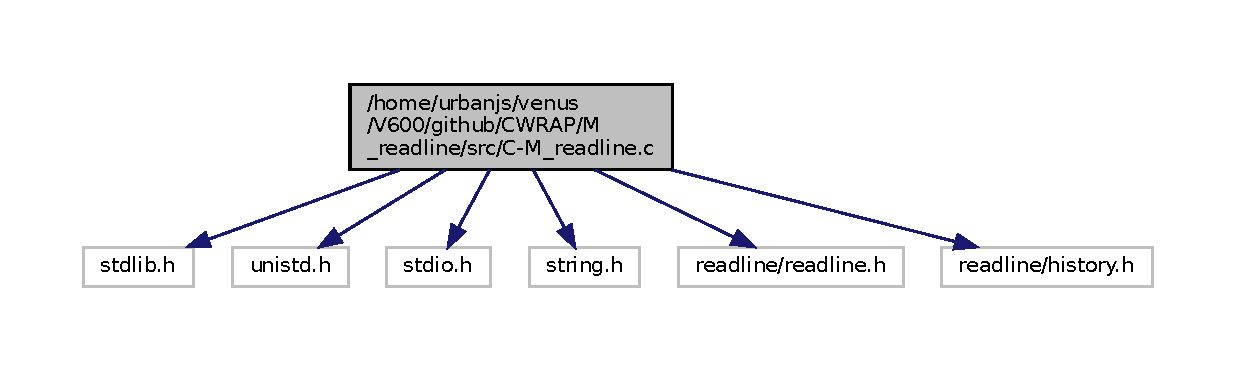
\includegraphics[width=350pt]{C-M__readline_8c__incl}
\end{center}
\end{figure}
\doxysubsection*{Functions}
\begin{DoxyCompactItemize}
\item 
void \mbox{\hyperlink{C-M__readline_8c_a80269900528c2ee04bf7cacb3a07ff40}{show\+\_\+history\+\_\+list}} ()
\item 
void \mbox{\hyperlink{C-M__readline_8c_a146edc06a54e833494378446131c6bcd}{F\+Creadline}} (int len, char $\ast$myline, char prompt\mbox{[}$\,$\mbox{]})
\end{DoxyCompactItemize}


\doxysubsection{Function Documentation}
\mbox{\Hypertarget{C-M__readline_8c_a146edc06a54e833494378446131c6bcd}\label{C-M__readline_8c_a146edc06a54e833494378446131c6bcd}} 
\index{C-\/M\_readline.c@{C-\/M\_readline.c}!FCreadline@{FCreadline}}
\index{FCreadline@{FCreadline}!C-\/M\_readline.c@{C-\/M\_readline.c}}
\doxysubsubsection{\texorpdfstring{FCreadline()}{FCreadline()}}
{\footnotesize\ttfamily void F\+Creadline (\begin{DoxyParamCaption}\item[{int}]{len,  }\item[{char $\ast$}]{myline,  }\item[{char}]{prompt\mbox{[}$\,$\mbox{]} }\end{DoxyParamCaption})}



References show\+\_\+history\+\_\+list().

Here is the call graph for this function\+:\nopagebreak
\begin{figure}[H]
\begin{center}
\leavevmode
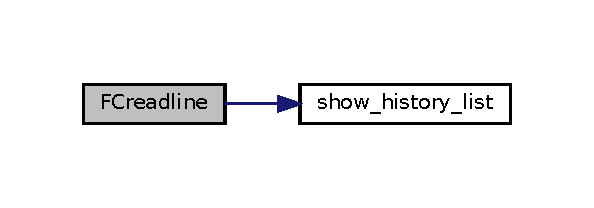
\includegraphics[width=286pt]{C-M__readline_8c_a146edc06a54e833494378446131c6bcd_cgraph}
\end{center}
\end{figure}
\mbox{\Hypertarget{C-M__readline_8c_a80269900528c2ee04bf7cacb3a07ff40}\label{C-M__readline_8c_a80269900528c2ee04bf7cacb3a07ff40}} 
\index{C-\/M\_readline.c@{C-\/M\_readline.c}!show\_history\_list@{show\_history\_list}}
\index{show\_history\_list@{show\_history\_list}!C-\/M\_readline.c@{C-\/M\_readline.c}}
\doxysubsubsection{\texorpdfstring{show\_history\_list()}{show\_history\_list()}}
{\footnotesize\ttfamily void show\+\_\+history\+\_\+list (\begin{DoxyParamCaption}{ }\end{DoxyParamCaption})}

Here is the caller graph for this function\+:\nopagebreak
\begin{figure}[H]
\begin{center}
\leavevmode
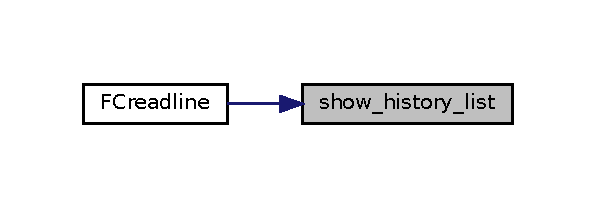
\includegraphics[width=286pt]{C-M__readline_8c_a80269900528c2ee04bf7cacb3a07ff40_icgraph}
\end{center}
\end{figure}

\hypertarget{M__readline_8f90}{}\section{/home/urbanjs/venus/\+V600/github/\+M\+\_\+readline/src/\+M\+\_\+readline.f90 File Reference}
\label{M__readline_8f90}\index{/home/urbanjs/venus/\+V600/github/\+M\+\_\+readline/src/\+M\+\_\+readline.\+f90@{/home/urbanjs/venus/\+V600/github/\+M\+\_\+readline/src/\+M\+\_\+readline.\+f90}}
\subsection*{Data Types}
\begin{DoxyCompactItemize}
\item 
interface \mbox{\hyperlink{interfacem__readline_1_1Freadline}{m\+\_\+readline\+::\+Freadline}}
\end{DoxyCompactItemize}
\subsection*{Modules}
\begin{DoxyCompactItemize}
\item 
module \mbox{\hyperlink{namespacem__readline}{m\+\_\+readline}}
\begin{DoxyCompactList}\small\item\em \subsubsection*{N\+A\+ME}

M\+\_\+readline(3fm) -\/ \mbox{[}M\+\_\+readline\mbox{]} Calling readline(3c) from Fortran (L\+I\+C\+E\+N\+SE\+:PD) \subsubsection*{S\+Y\+N\+O\+P\+S\+IS}\end{DoxyCompactList}\end{DoxyCompactItemize}
\subsection*{Functions/\+Subroutines}
\begin{DoxyCompactItemize}
\item 
subroutine, public \mbox{\hyperlink{namespacem__readline_a6eae368d34bd43ead64623b2d6d10ae0}{m\+\_\+readline\+::system\+\_\+readline}} (line, prompt)
\begin{DoxyCompactList}\small\item\em \subsubsection*{N\+A\+ME}

system\+\_\+readline(3f) -\/ \mbox{[}M\+\_\+readline\mbox{]} Call readline(3c) from Fortran (L\+I\+C\+E\+N\+SE\+:PD) \subsubsection*{S\+Y\+N\+O\+P\+S\+IS}\end{DoxyCompactList}\end{DoxyCompactItemize}

\hypertarget{mainpage_8txt}{}\doxysection{/home/urbanjs/venus/\+V600/github/\+C\+W\+R\+A\+P/\+M\+\_\+readline/src/mainpage.txt File Reference}
\label{mainpage_8txt}\index{/home/urbanjs/venus/V600/github/CWRAP/M\_readline/src/mainpage.txt@{/home/urbanjs/venus/V600/github/CWRAP/M\_readline/src/mainpage.txt}}

%--- End generated contents ---

% Index
\backmatter
\newpage
\phantomsection
\clearemptydoublepage
\addcontentsline{toc}{chapter}{Index}
\printindex

\end{document}
